\chapter[Tau leptons][Tau leptons]{Tau leptons}

\begin{quote}
  Tau leptons and their signature in the ATLAS detector are described.
\end{quote}

\section{Tau leptons}
\label{sec:taus-theory}

\begin{figure}[tp]
  \centering
  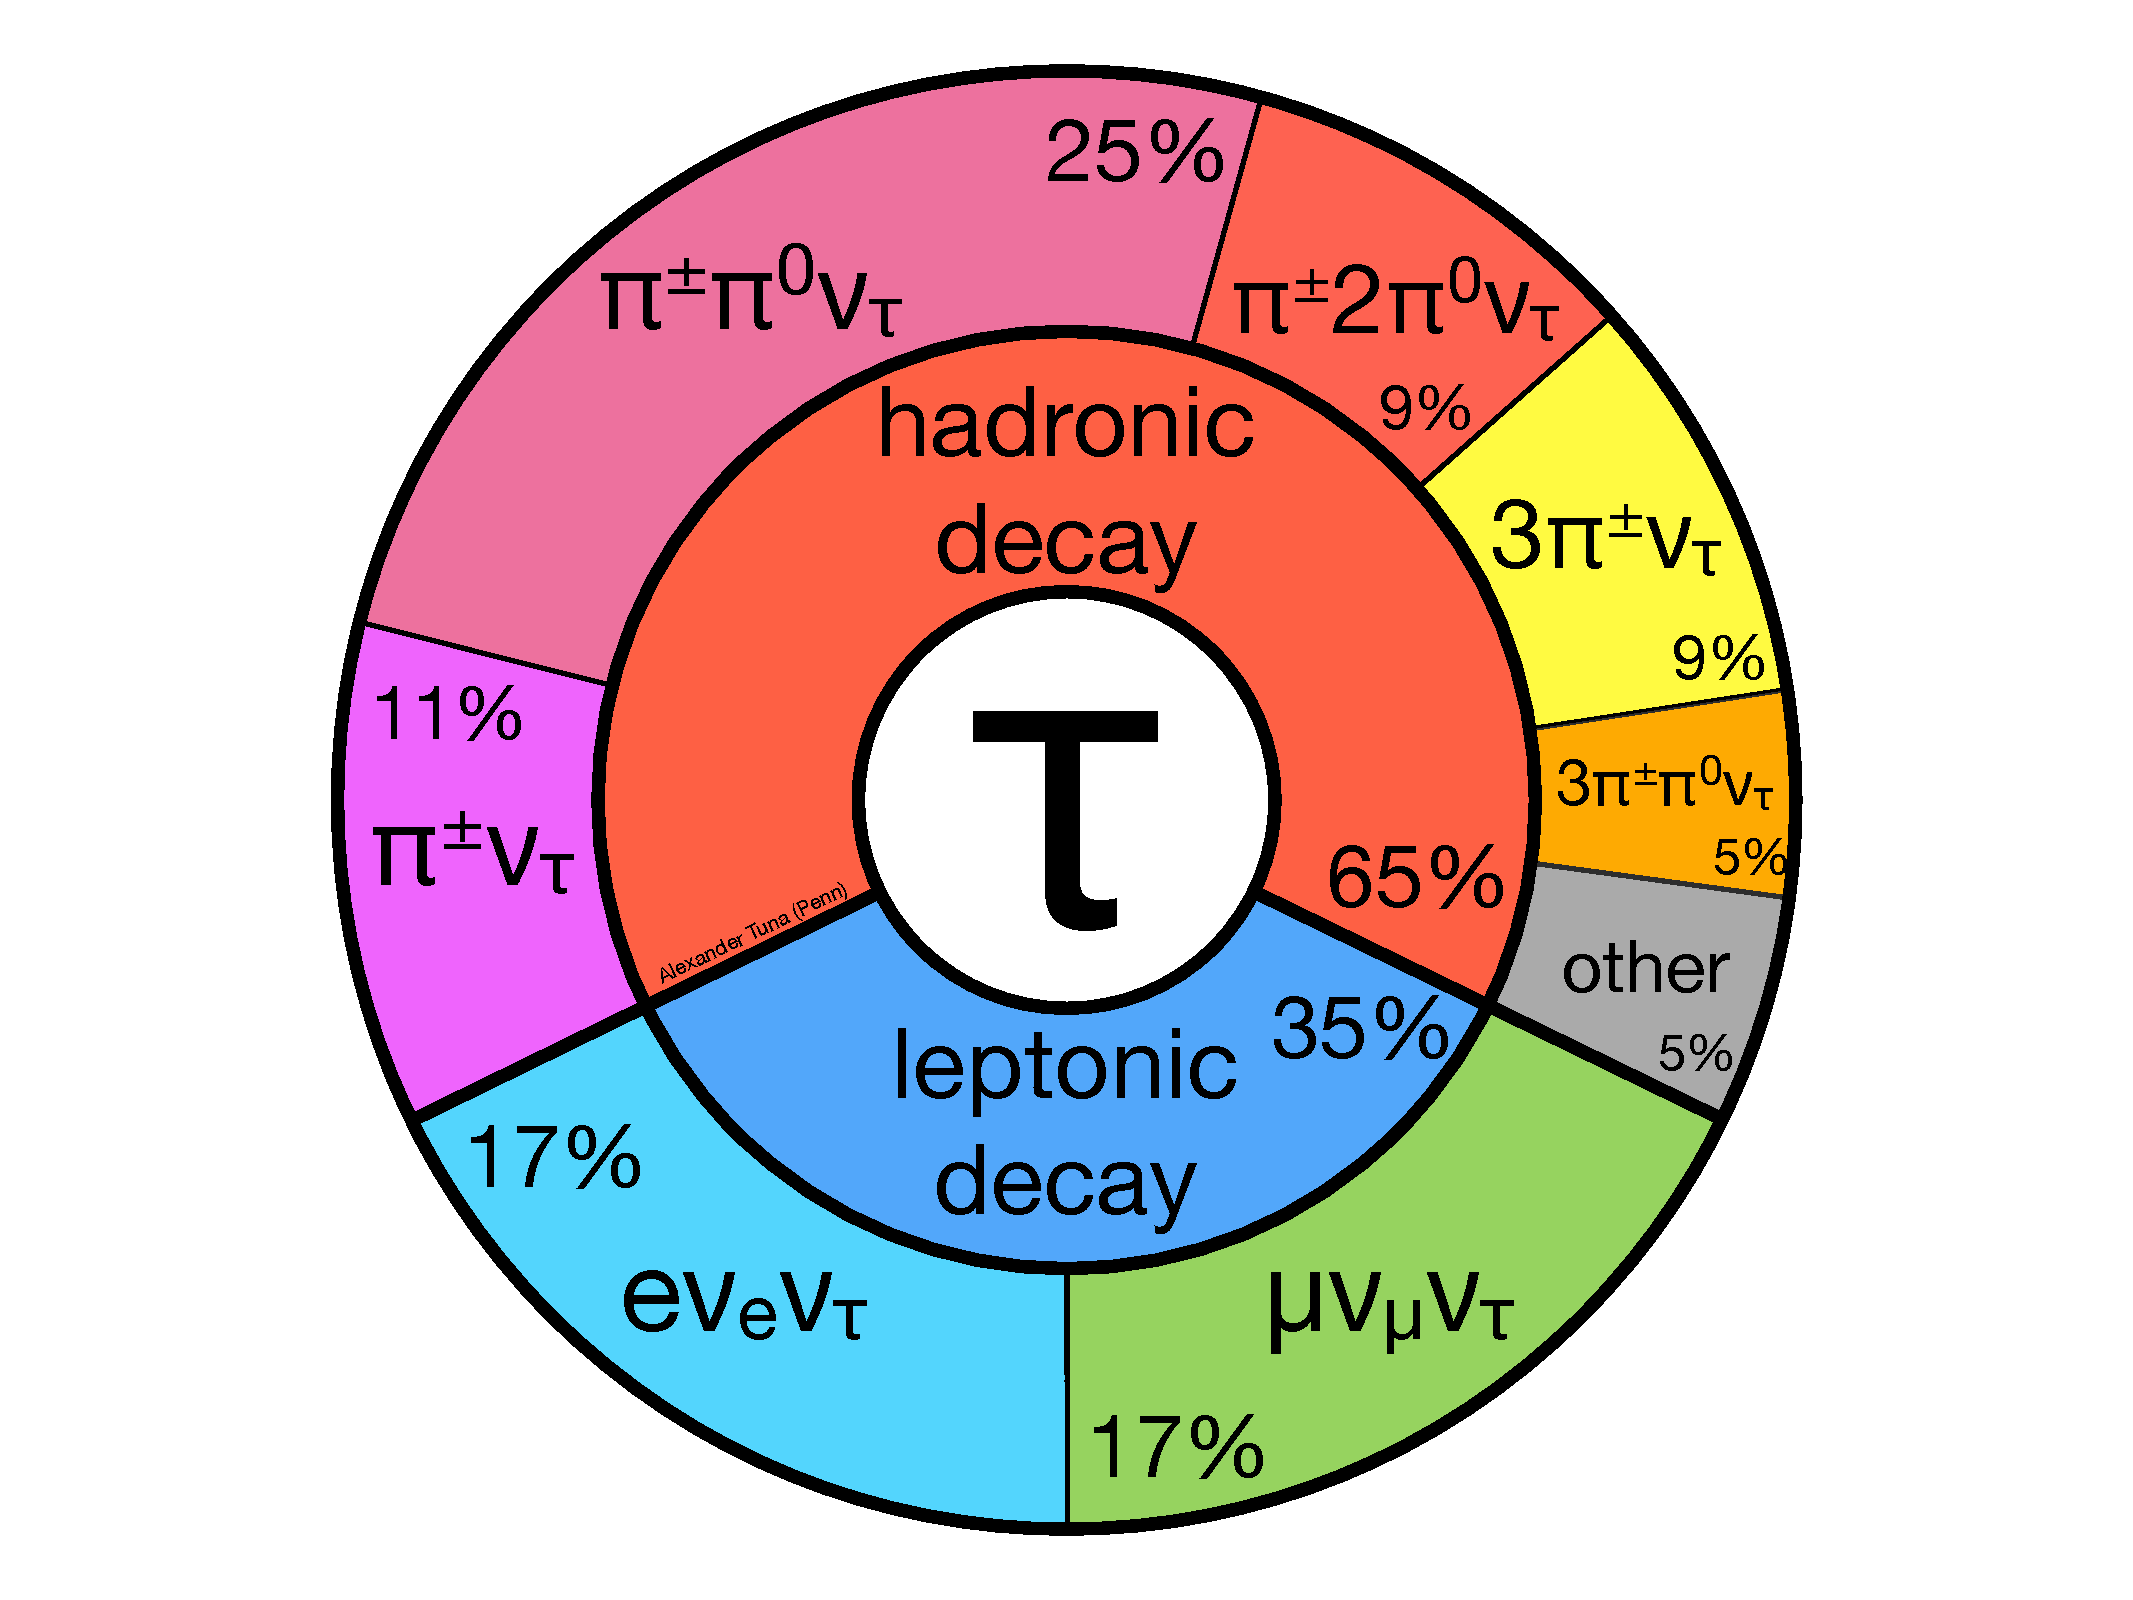
\includegraphics[width=0.48\textwidth]{figures/piecharts/taudecay}
  \caption{Variables.}
  \label{fig:taus-decaypie}
\end{figure}

\section{Hadronic tau decays, $\tauh$}
\label{sec:taus-jetfakes}

\begin{figure}[tp]
  \centering
  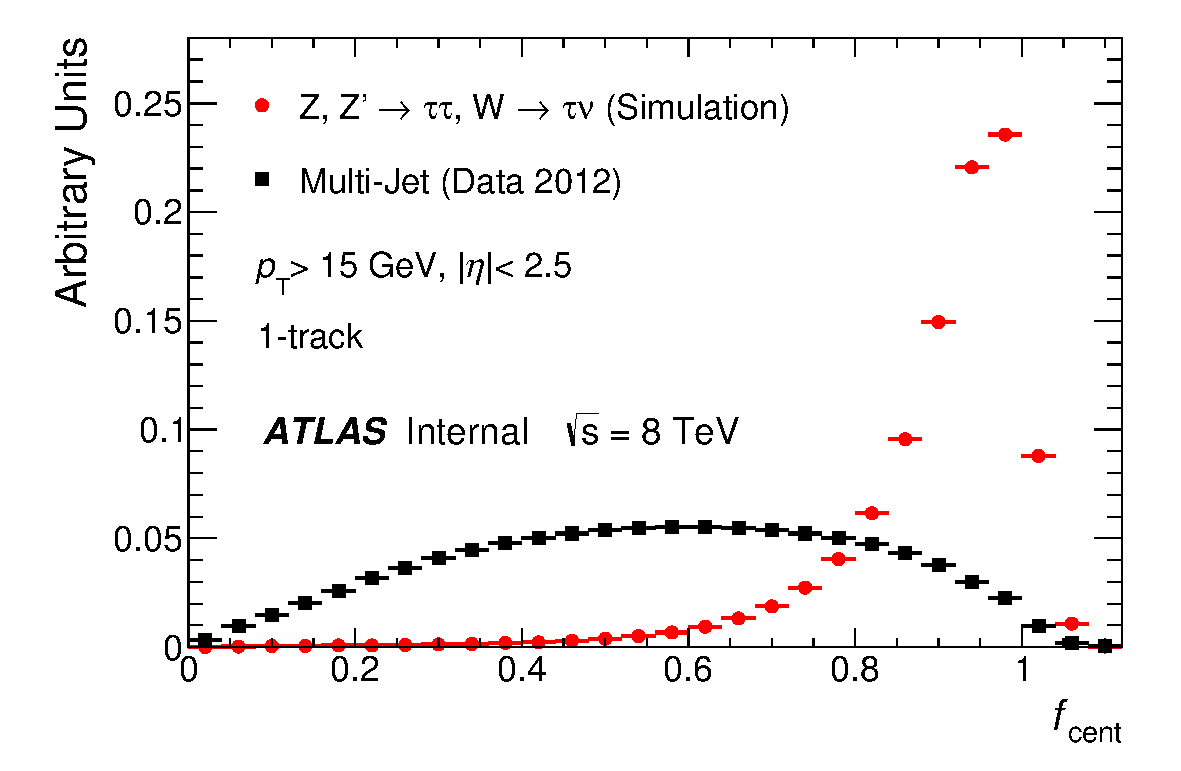
\includegraphics[width=0.48\textwidth]{figures/PERF-2013-06_tmp/centFrac_1p}
  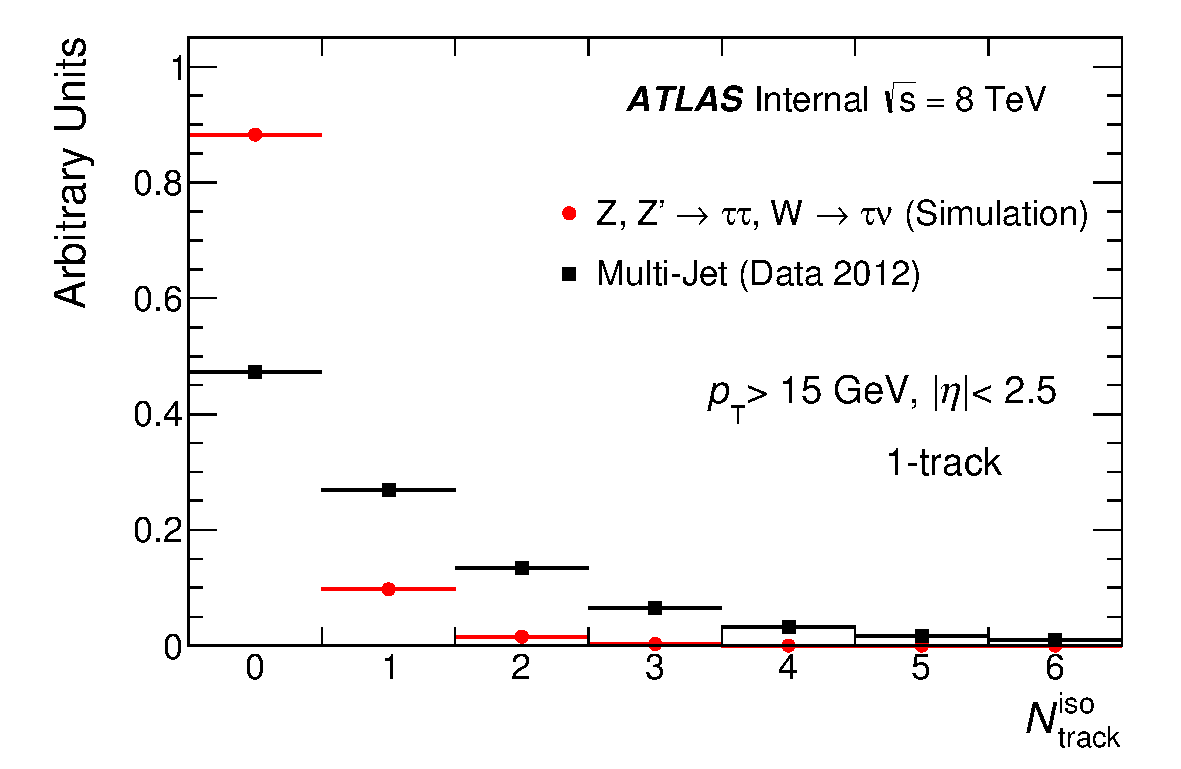
\includegraphics[width=0.48\textwidth]{figures/PERF-2013-06_tmp/wideTrk_n_1p}
  \caption{Variables.}
  \label{fig:taus-id1p}
\end{figure}

\begin{figure}[tp]
  \centering
  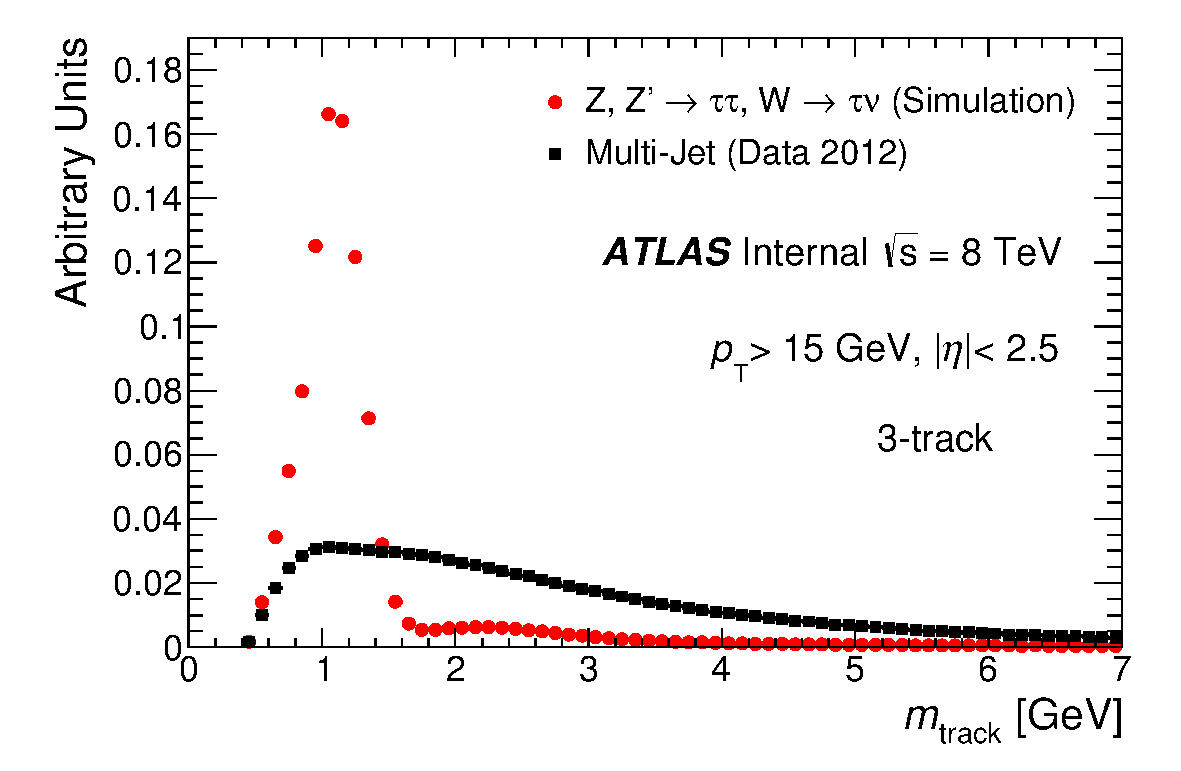
\includegraphics[width=0.48\textwidth]{figures/PERF-2013-06_tmp/massTrkSys_3p}
  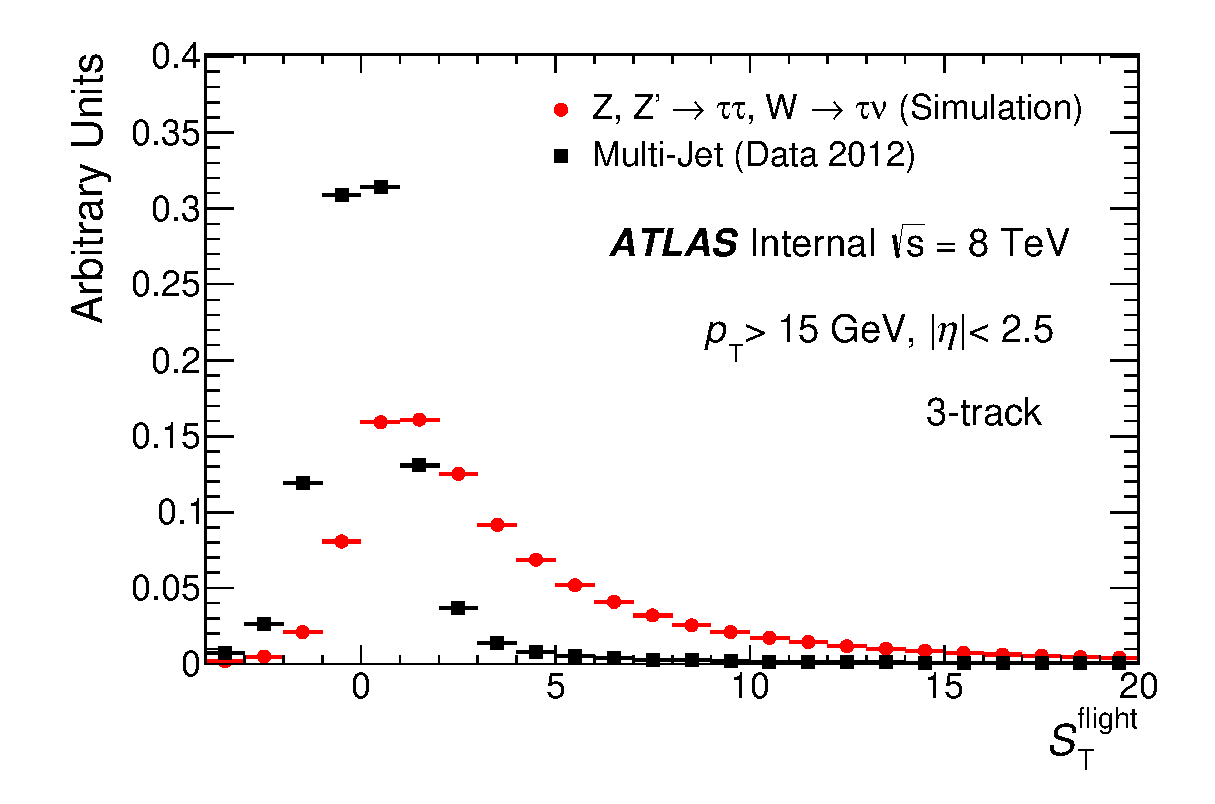
\includegraphics[width=0.48\textwidth]{figures/PERF-2013-06_tmp/trFlightPathSig_3p}
  \caption{Variables.}
  \label{fig:taus-id3p}
\end{figure}

\begin{figure}[tp]
  \centering
  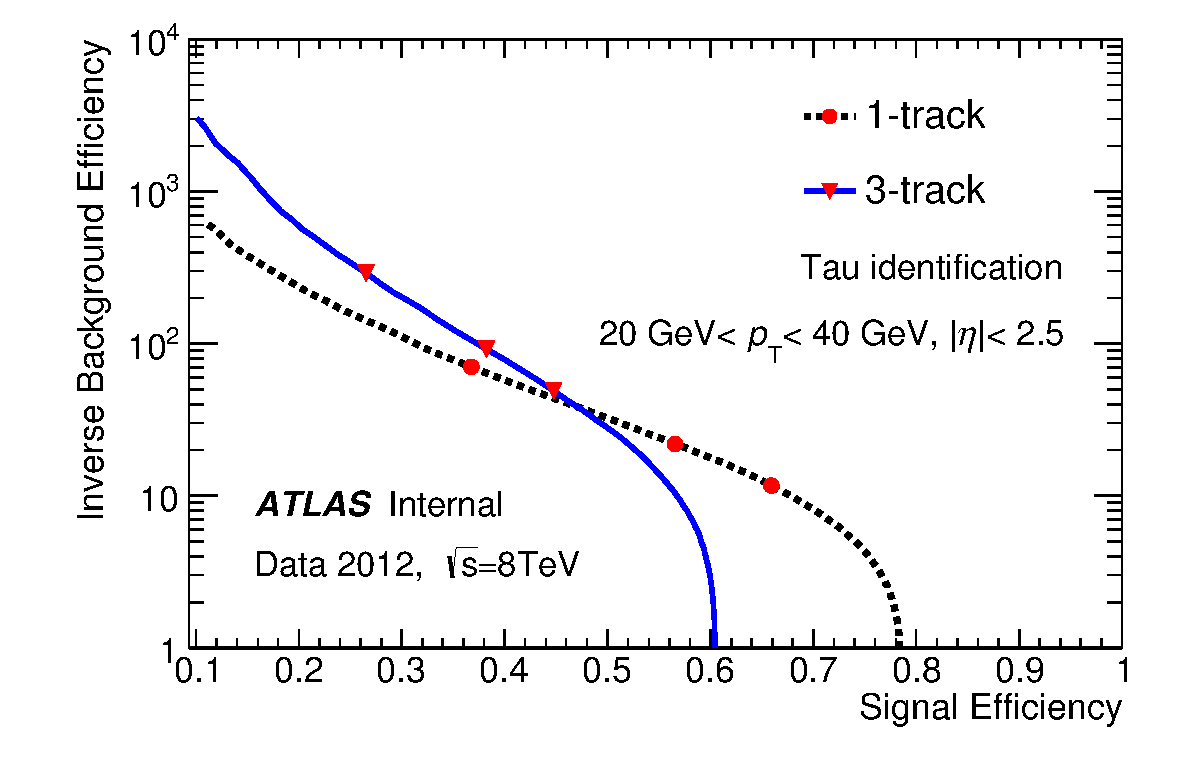
\includegraphics[width=0.48\textwidth]{figures/PERF-2013-06_tmp/roc_lowpt}
  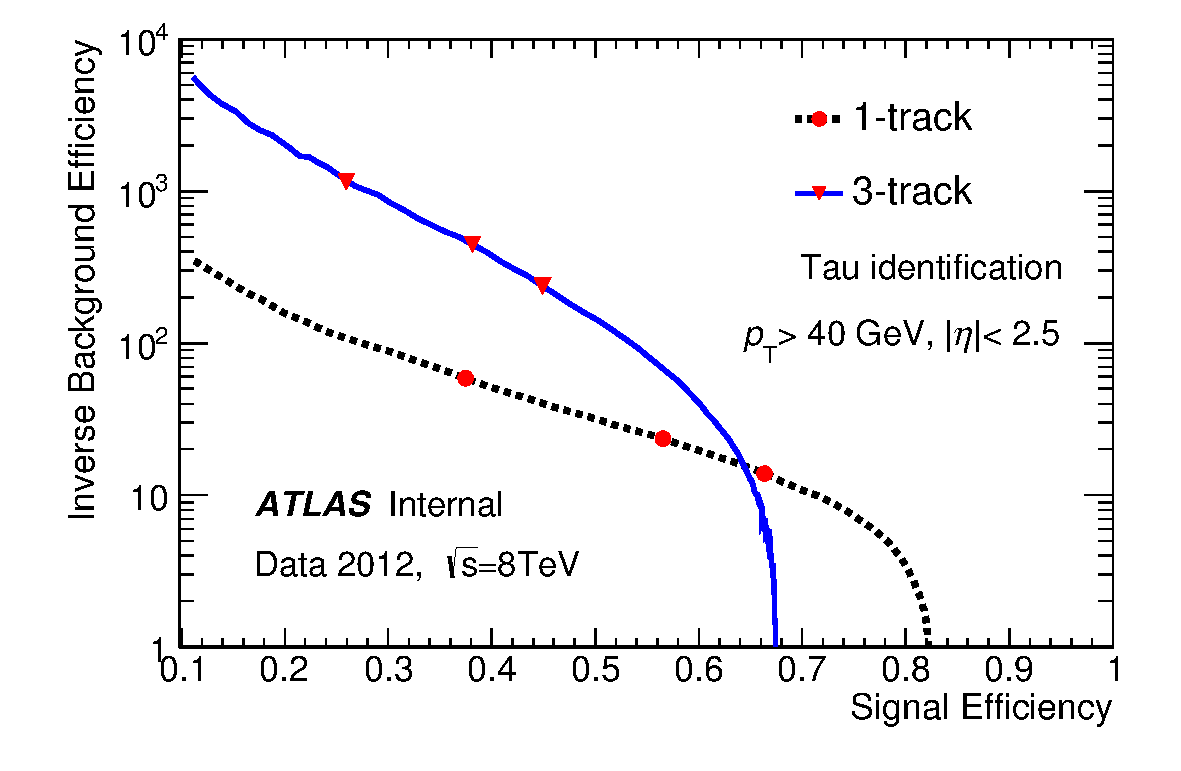
\includegraphics[width=0.48\textwidth]{figures/PERF-2013-06_tmp/roc_highpt}
  \caption{Variables.}
  \label{fig:taus-idroc}
\end{figure}

\section{Leptons mis-identified as $\tauh$}
\label{sec:taus-leptonfakes}

\begin{figure}[tp]
  \centering
  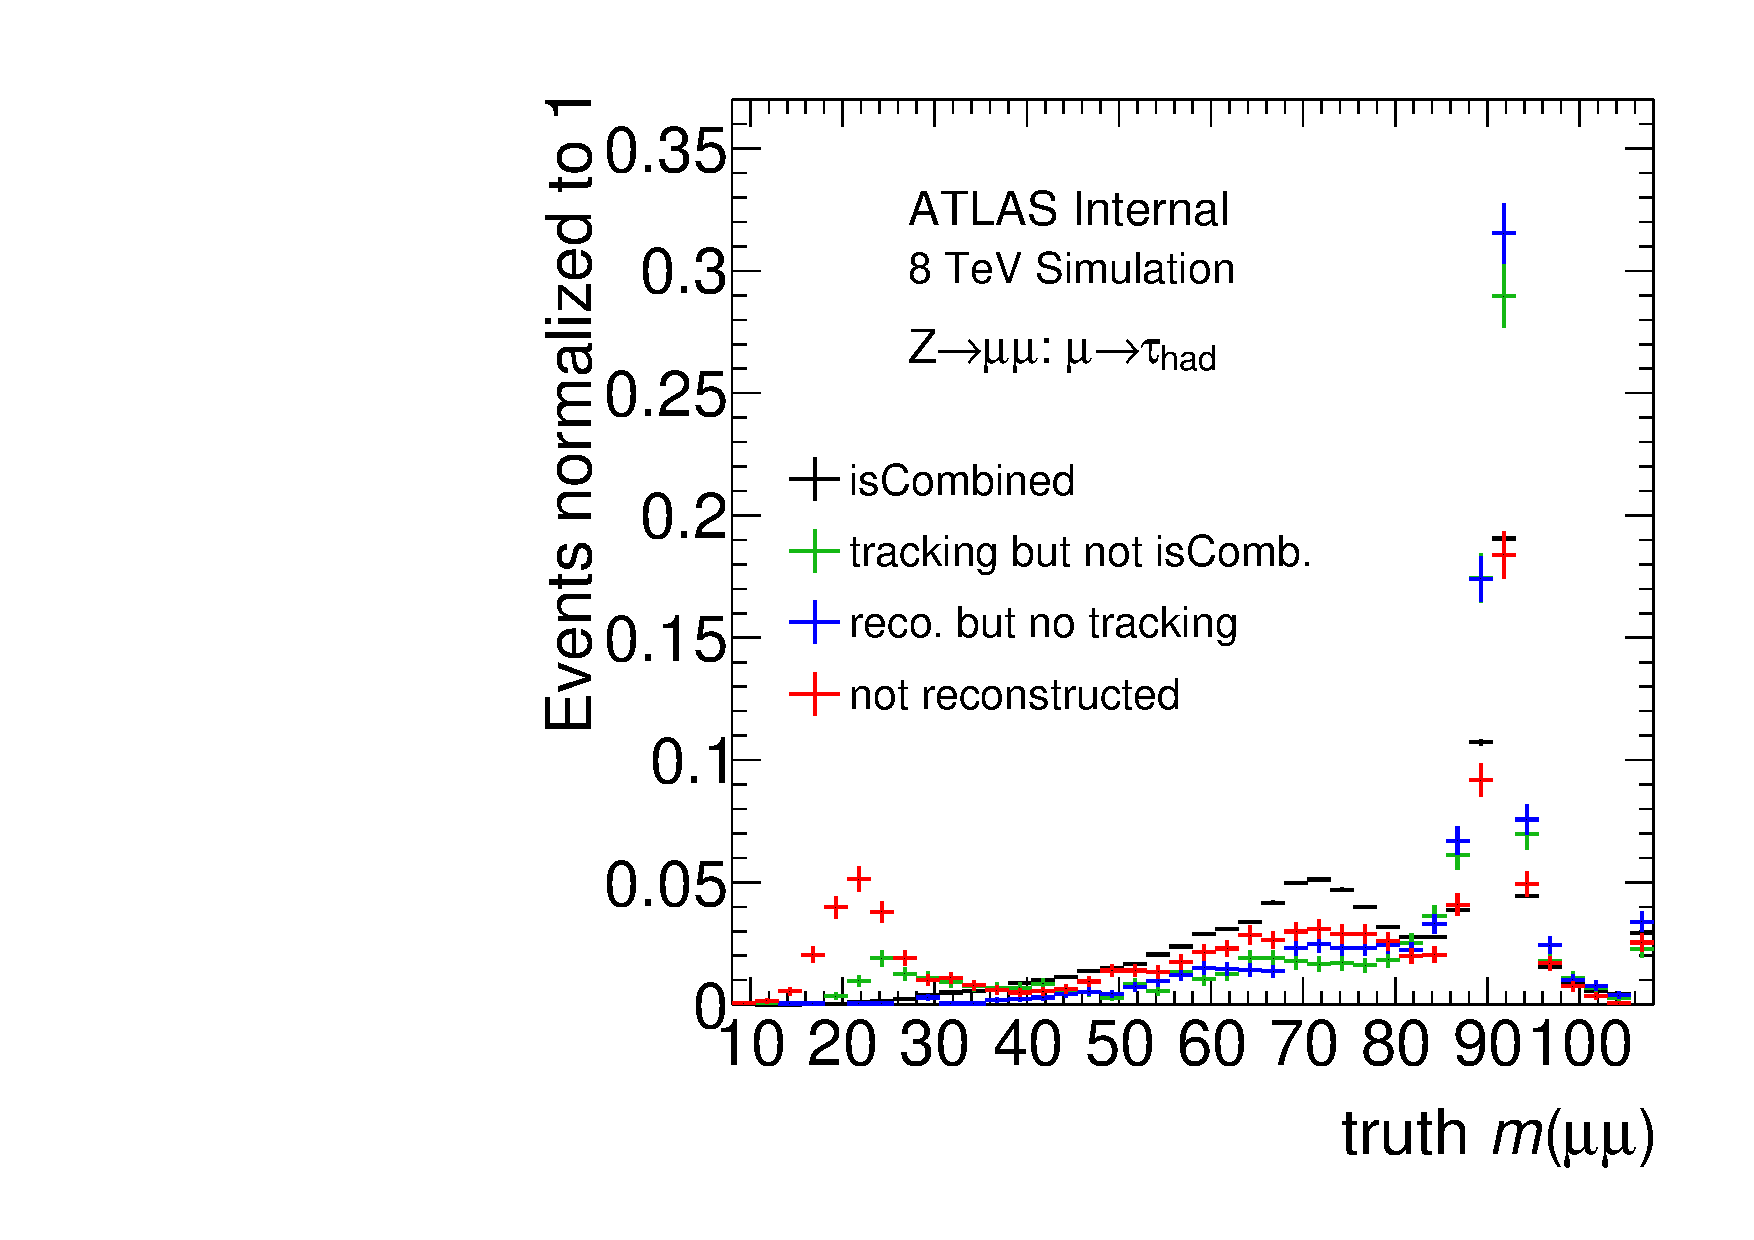
\includegraphics[width=0.48\textwidth]{figures/tauperformance/muonfakes_mll}
  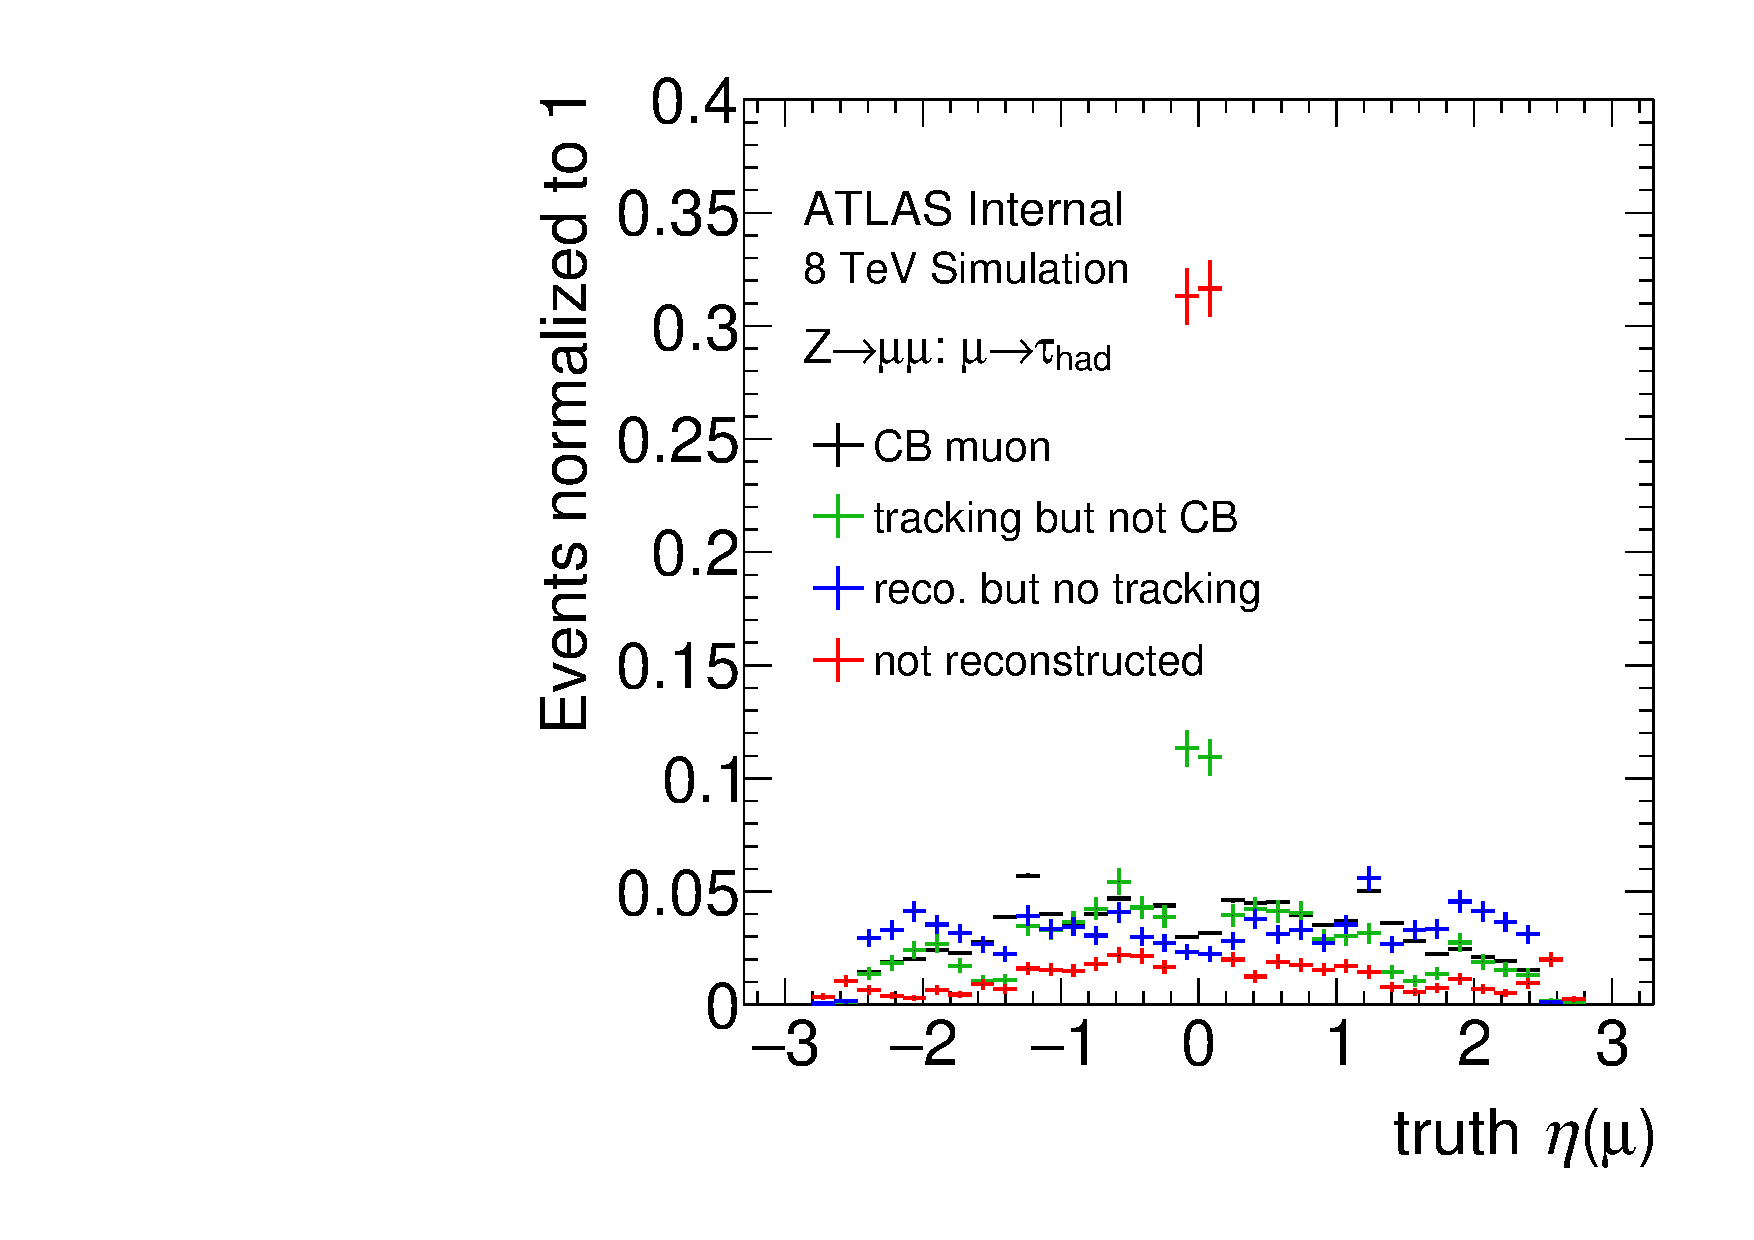
\includegraphics[width=0.48\textwidth]{figures/tauperformance/muonfakes_eta}
  \caption{Variables.}
  \label{fig:taus-muonfakes1}
\end{figure}

\begin{figure}[tp]
  \centering
  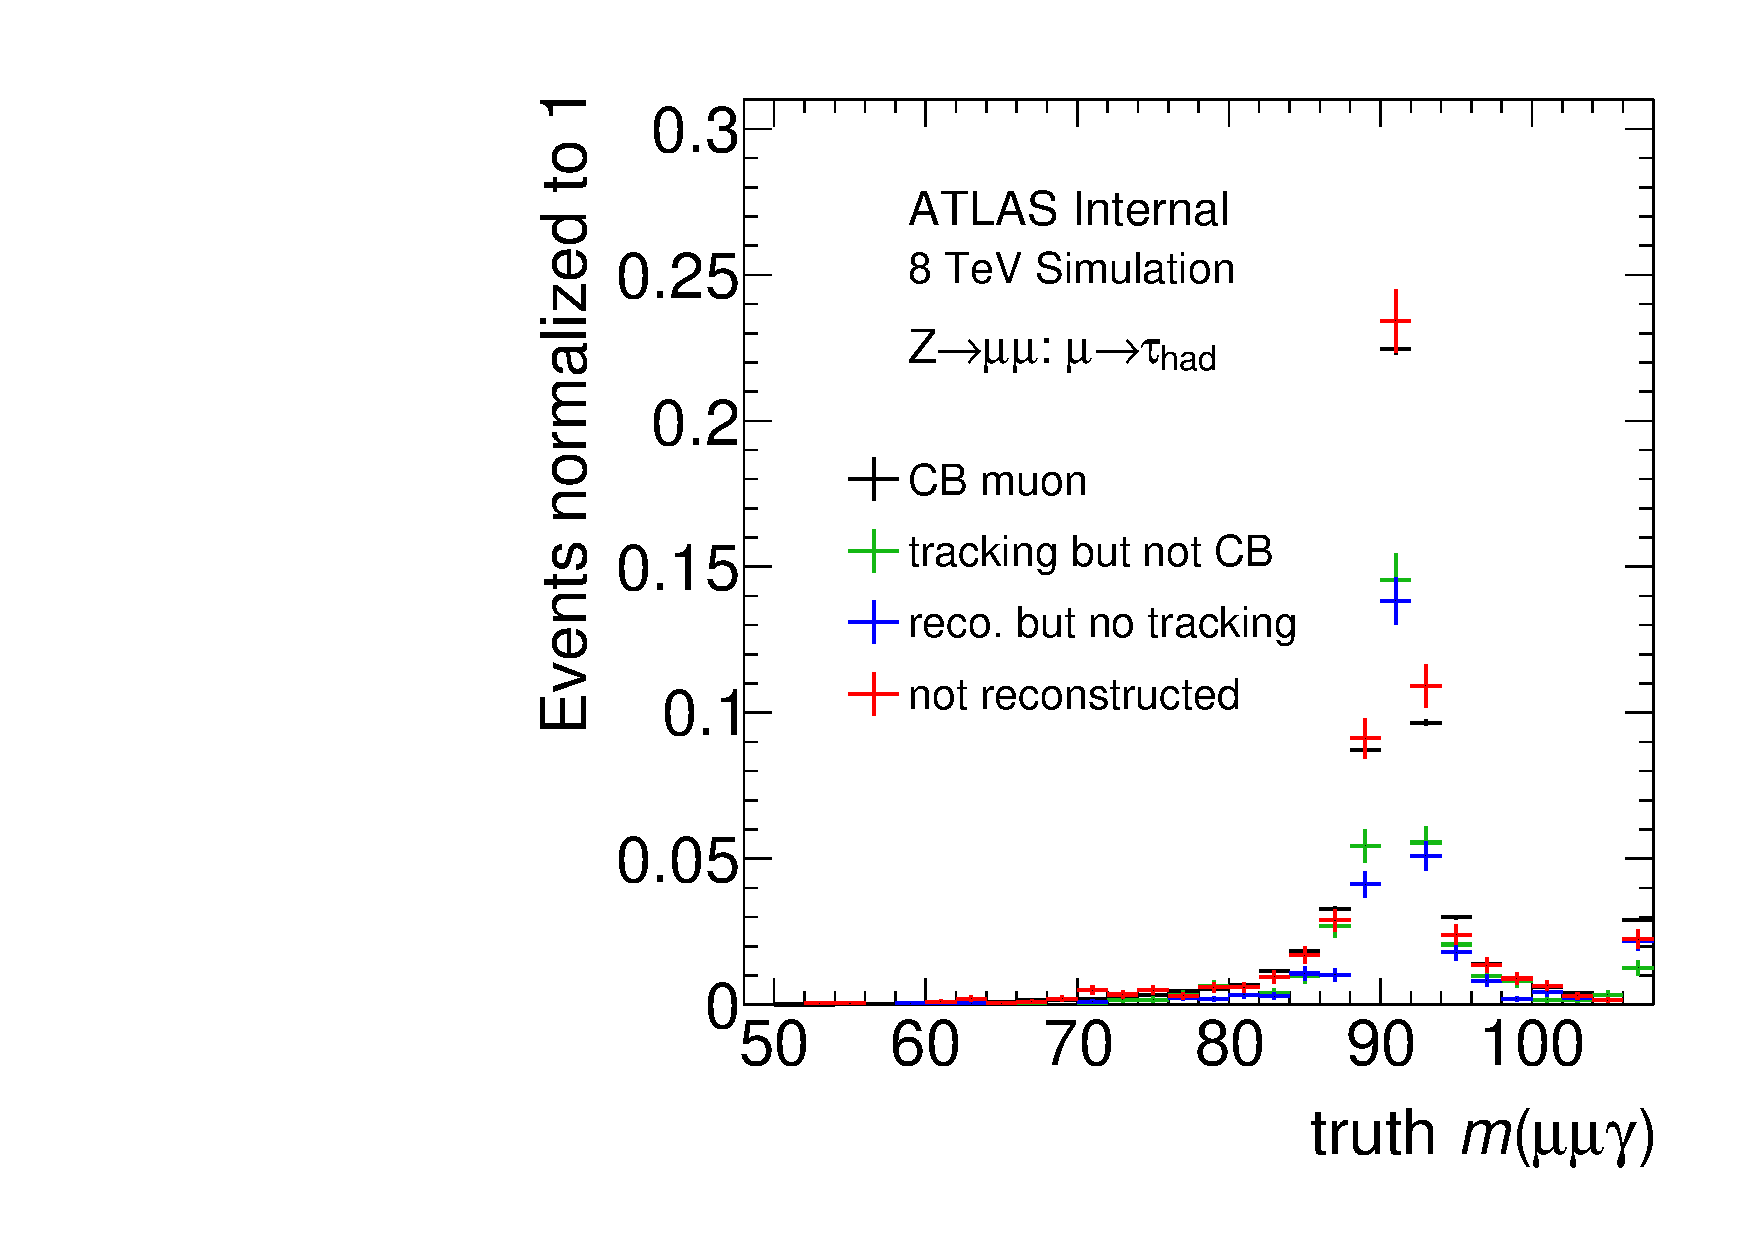
\includegraphics[width=0.48\textwidth]{figures/tauperformance/muonfakes_mlly}
  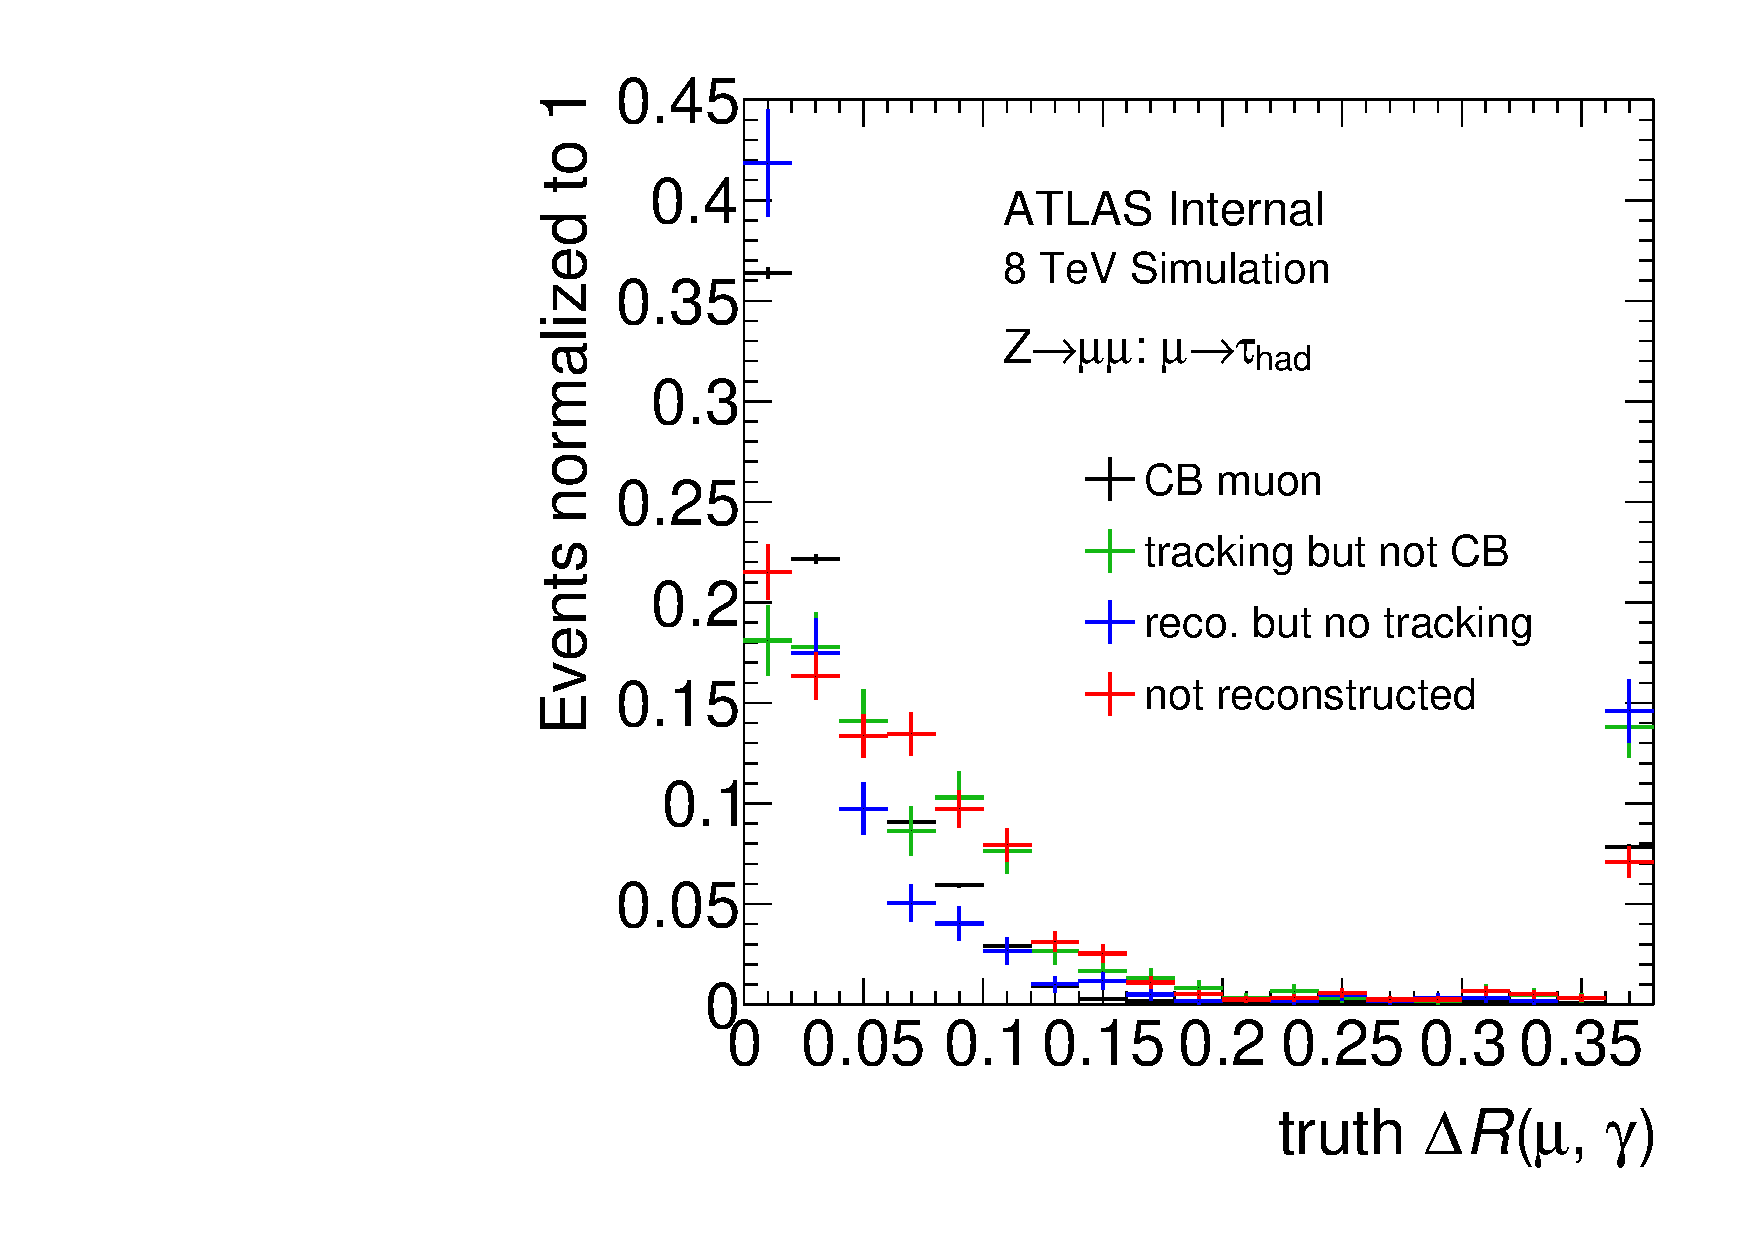
\includegraphics[width=0.48\textwidth]{figures/tauperformance/muonfakes_dR}
  \caption{Variables.}
  \label{fig:taus-muonfakes2}
\end{figure}

\begin{figure}[tp]
  \centering
  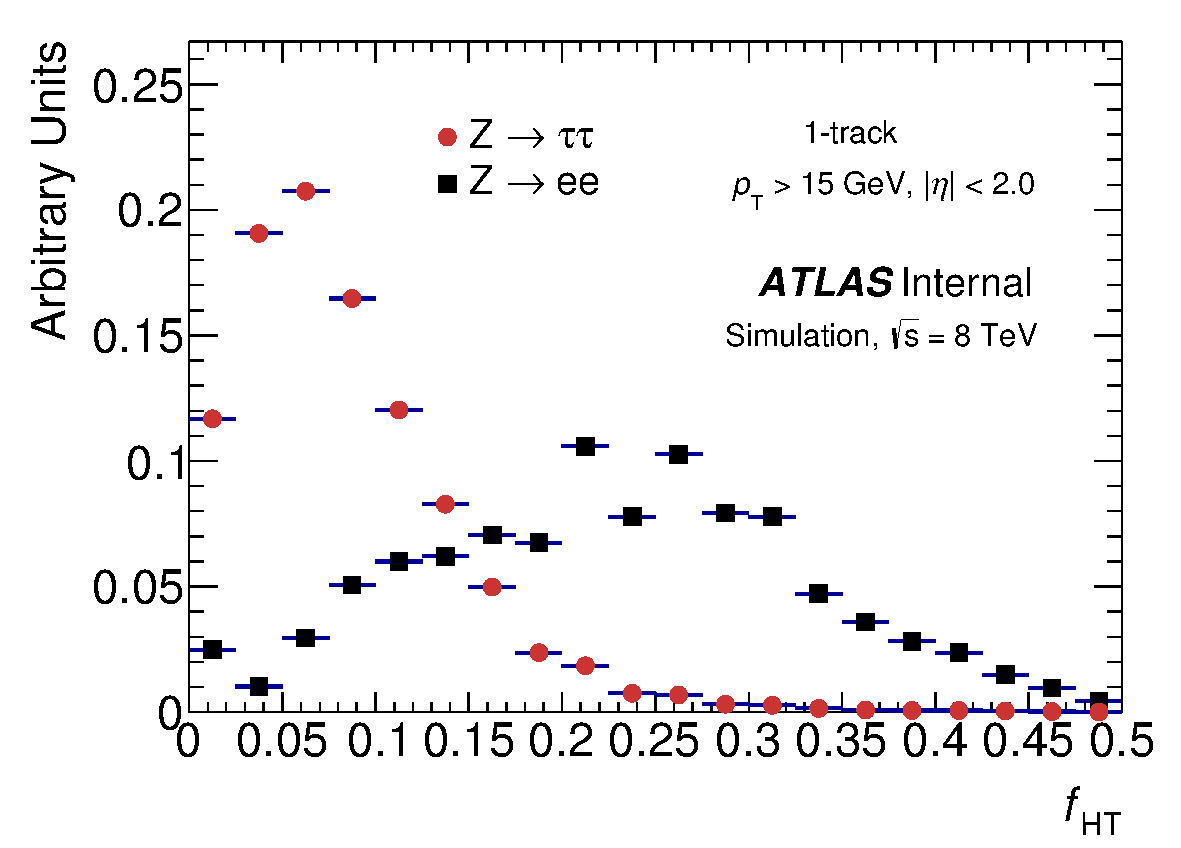
\includegraphics[width=0.48\textwidth]{figures/PERF-2013-06_tmp/TRTHTOverLT_LeadTrk}
  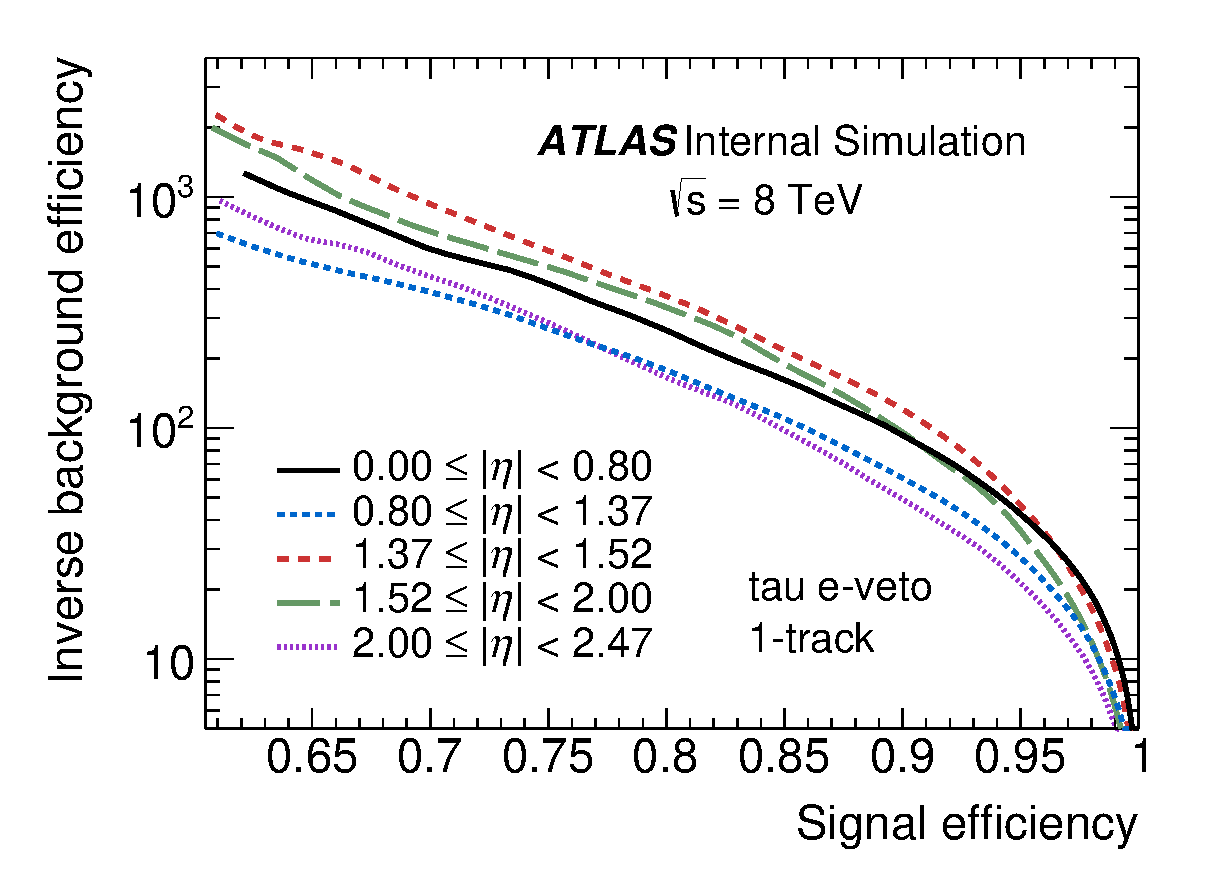
\includegraphics[width=0.48\textwidth]{figures/PERF-2013-06_tmp/ROC_ymin5_smoothcurve}
  \caption{Variables.}
  \label{fig:taus-electronfakes1}
\end{figure}

\begin{figure}[tp]
  \centering
  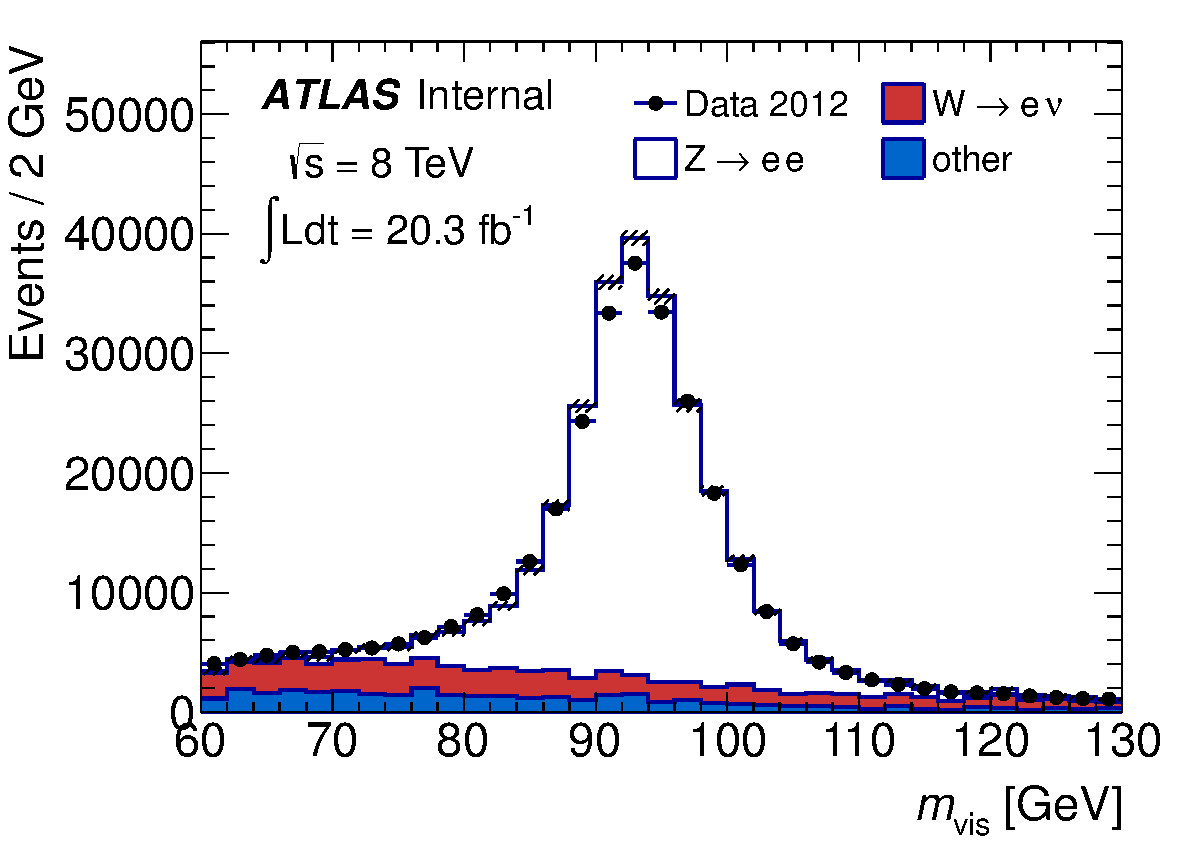
\includegraphics[width=0.48\textwidth]{figures/PERF-2013-06_tmp/eveto_mvis_mediumID_loosePPOLR_noeveto}
  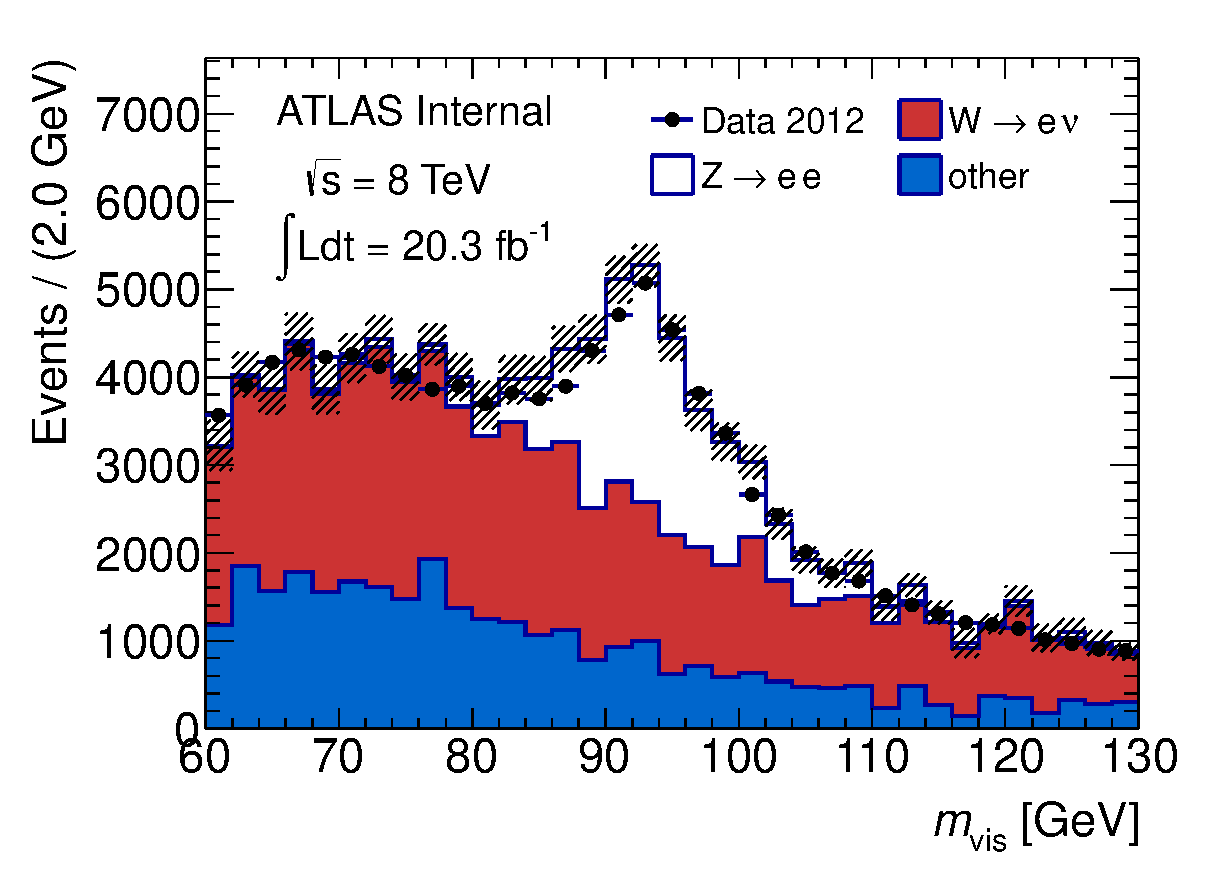
\includegraphics[width=0.48\textwidth]{figures/PERF-2013-06_tmp/eveto_mvis_mediumID_loosePPOLR_looseeveto}
  \caption{Variables.}
  \label{fig:taus-electronfakes2}
\end{figure}


